\section{Introduction}
\begin{frame}
\frametitle{Portfolio Management System}
\begin{columns}
\begin{column}{0.55\textwidth}
\begin{block}{Portfolio}
Collection of financial investments
\end{block}
\begin{block}{Portfolio Management System}
A system produces portfolios based on investment universe, the market, and investor preference
\end{block}
\end{column}
\begin{column}{0.45\textwidth}
\begin{center}
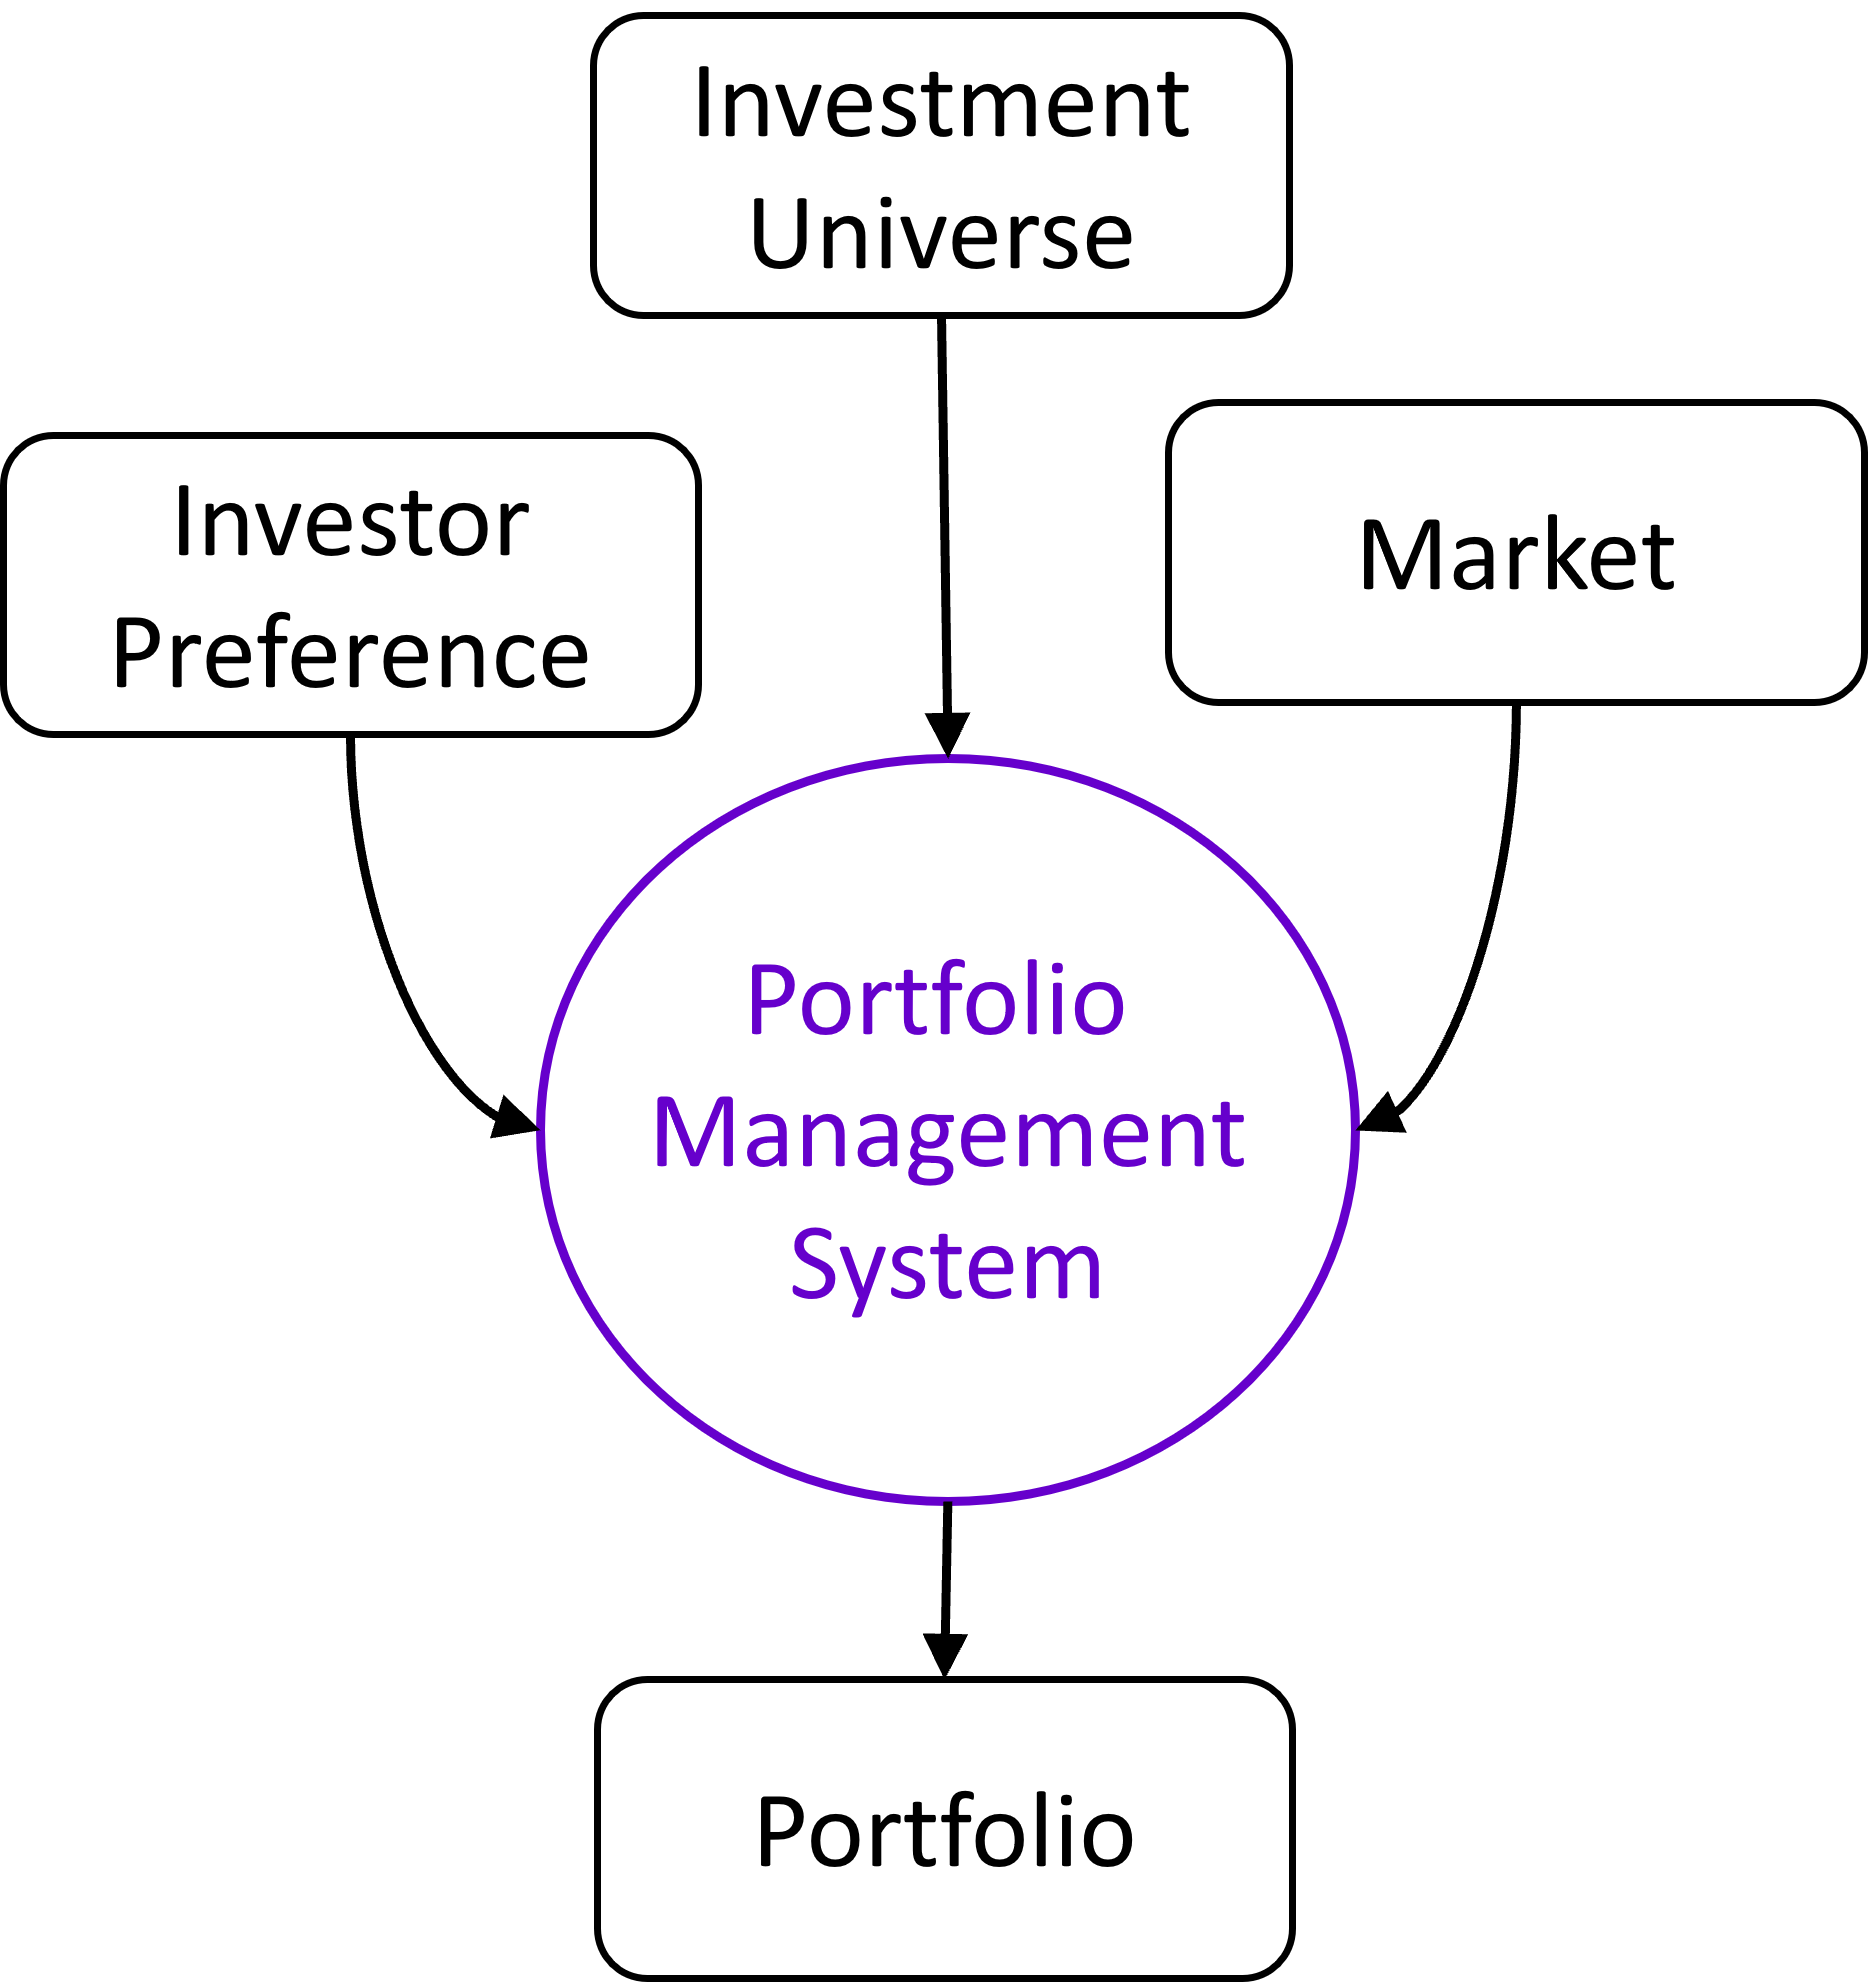
\includegraphics[width=4.8cm]{images/portfolio_management_system.png}
\end{center}
\end{column}
\end{columns}
\end{frame}







\begin{frame}
\frametitle{Supervised Learning Forecast System}
\begin{columns}
\begin{column}{0.55\textwidth}
\begin{itemize}
\item
Model trained with labeled data. 
The effects of transaction costs and tax are not considered.
\item
The Trading System in the next stage usually does not use inputs to the Forecast System, resulting in loss of information.
\end{itemize}
\end{column}
\begin{column}{0.45\textwidth}
\begin{center}
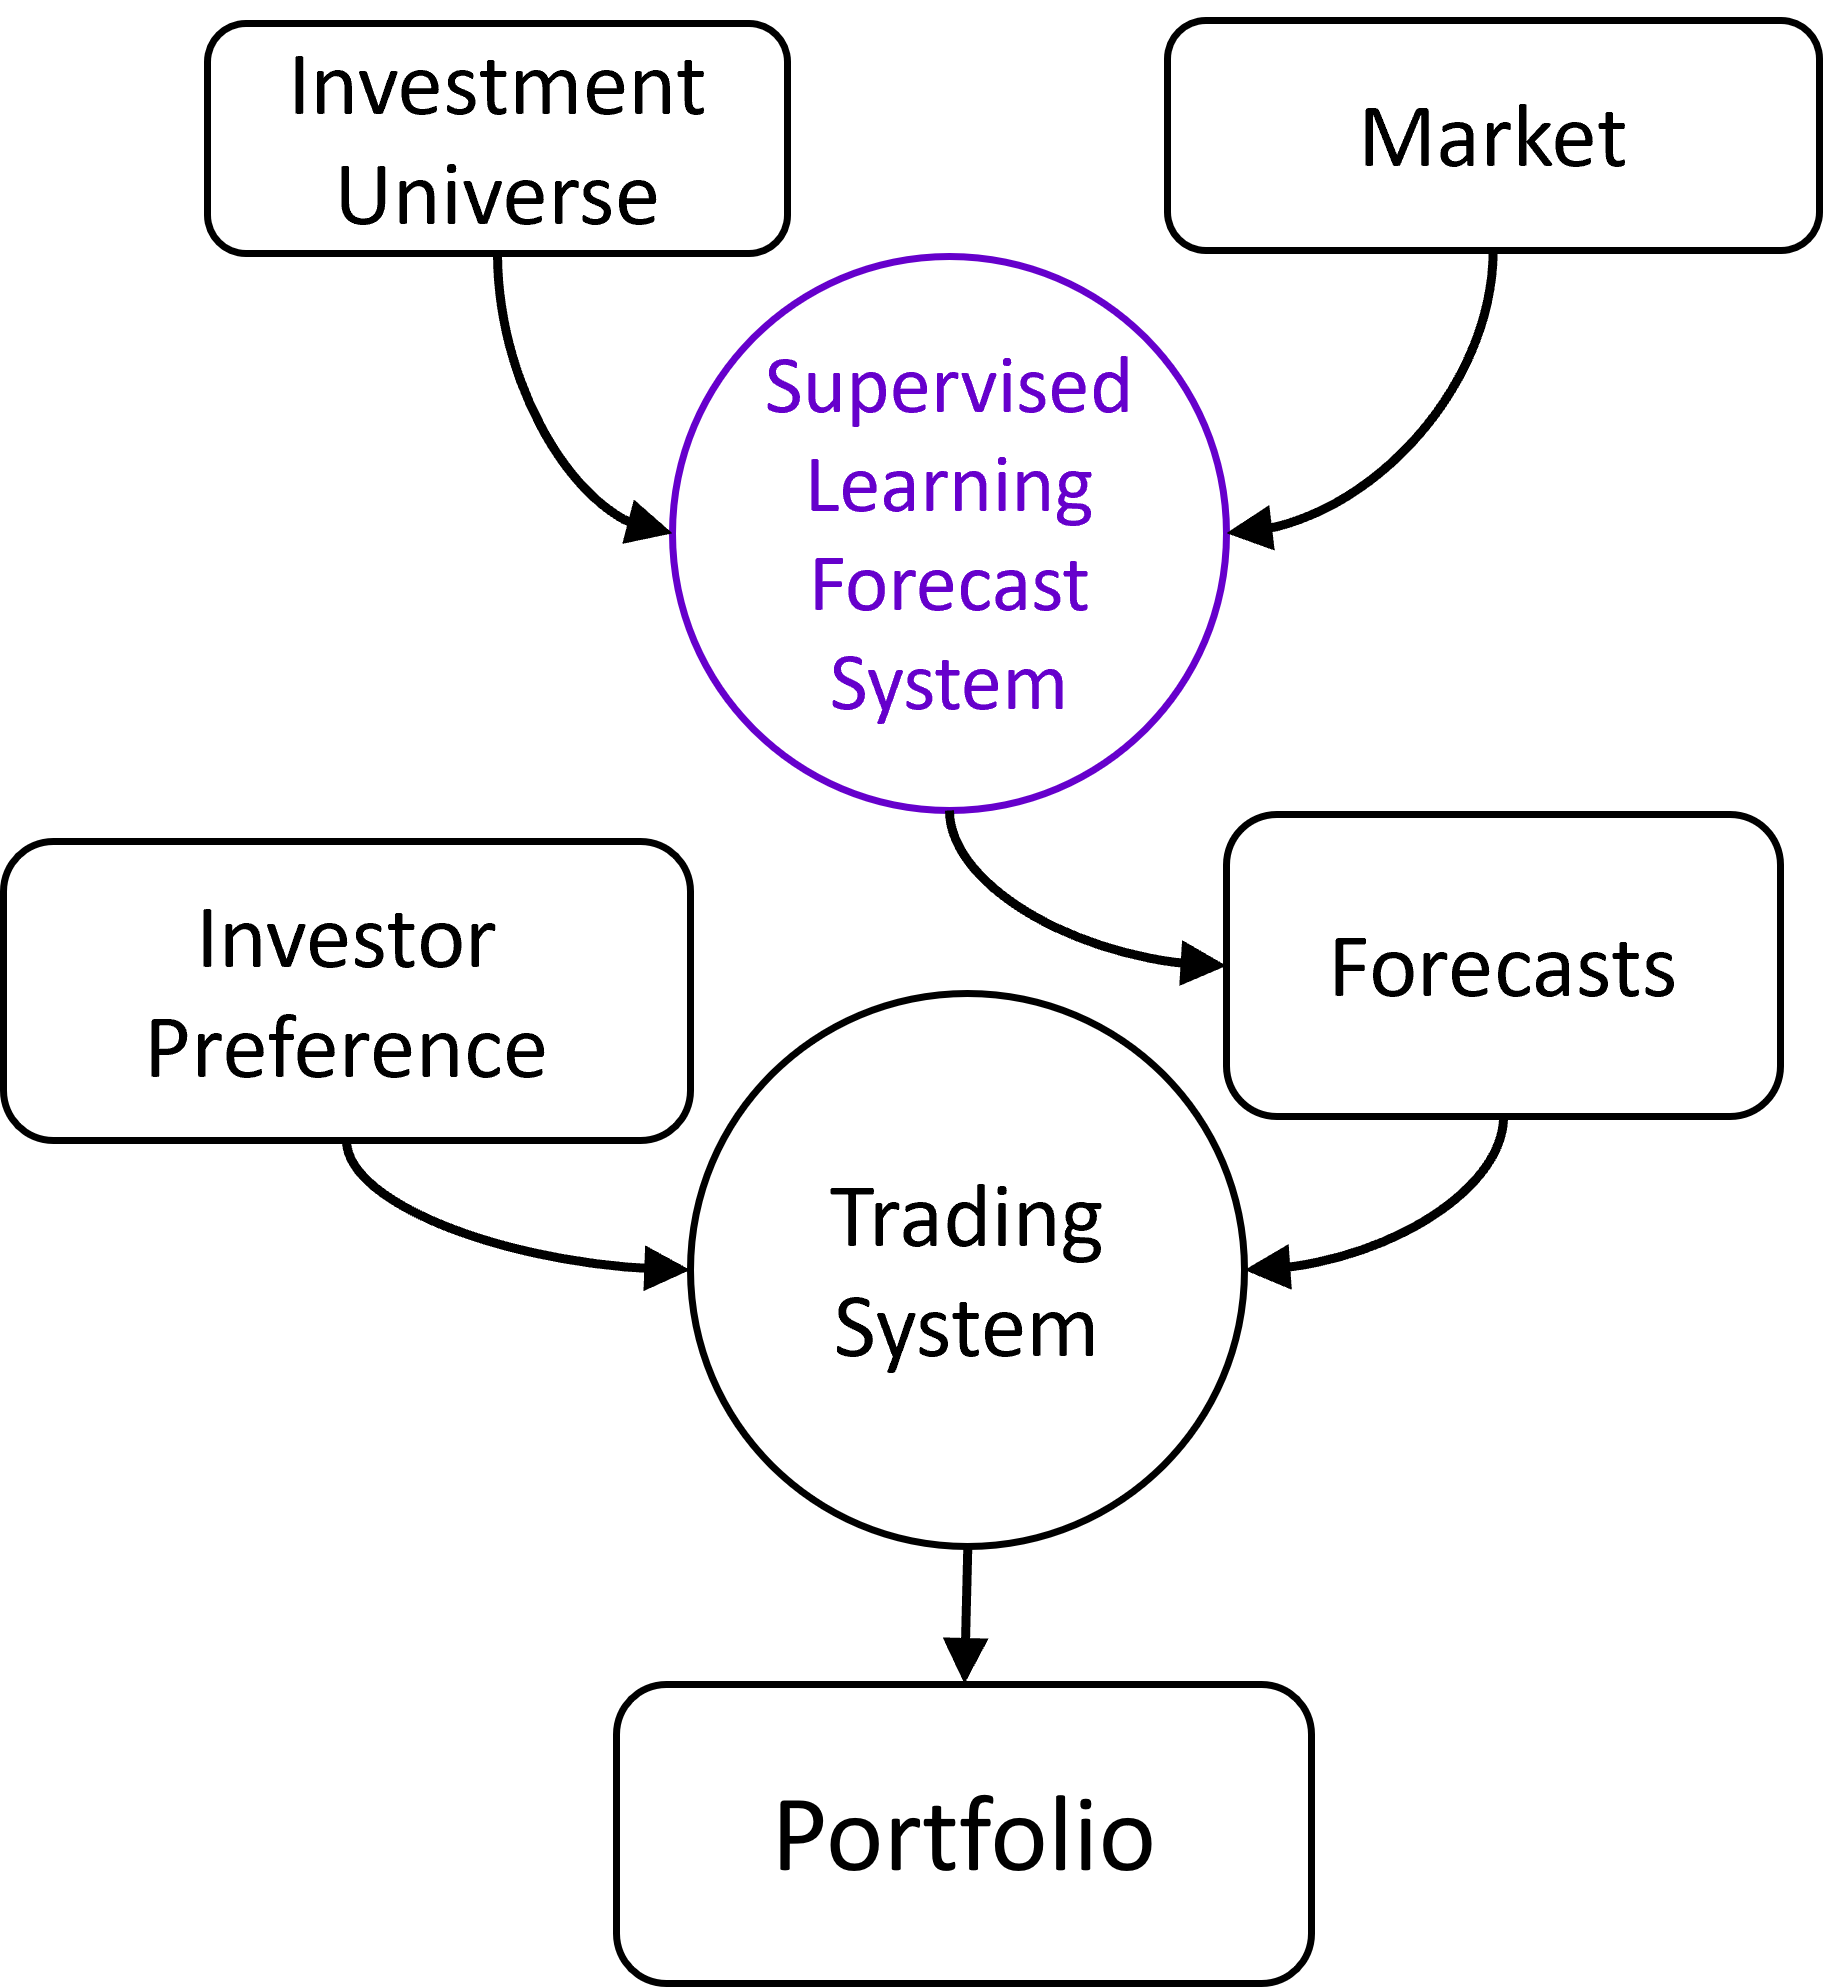
\includegraphics[width=4.8cm]{images/supervised_learning.png}
\end{center}
\end{column}
\end{columns}
\end{frame}



\begin{frame}
\frametitle{Reinforcement Learning (RL) based System}
\begin{columns}
\begin{column}{0.55\textwidth}
\begin{itemize}
\item
Optimize objective function directly without performance forecast.
\item
The effects of transaction costs and tax are considered.
\item
\alert
{To our knowledge, few RL-based Portfolio Management Systems incorporate with investor preference.}
\end{itemize}
\end{column}
\begin{column}{0.45\textwidth}
\begin{center}
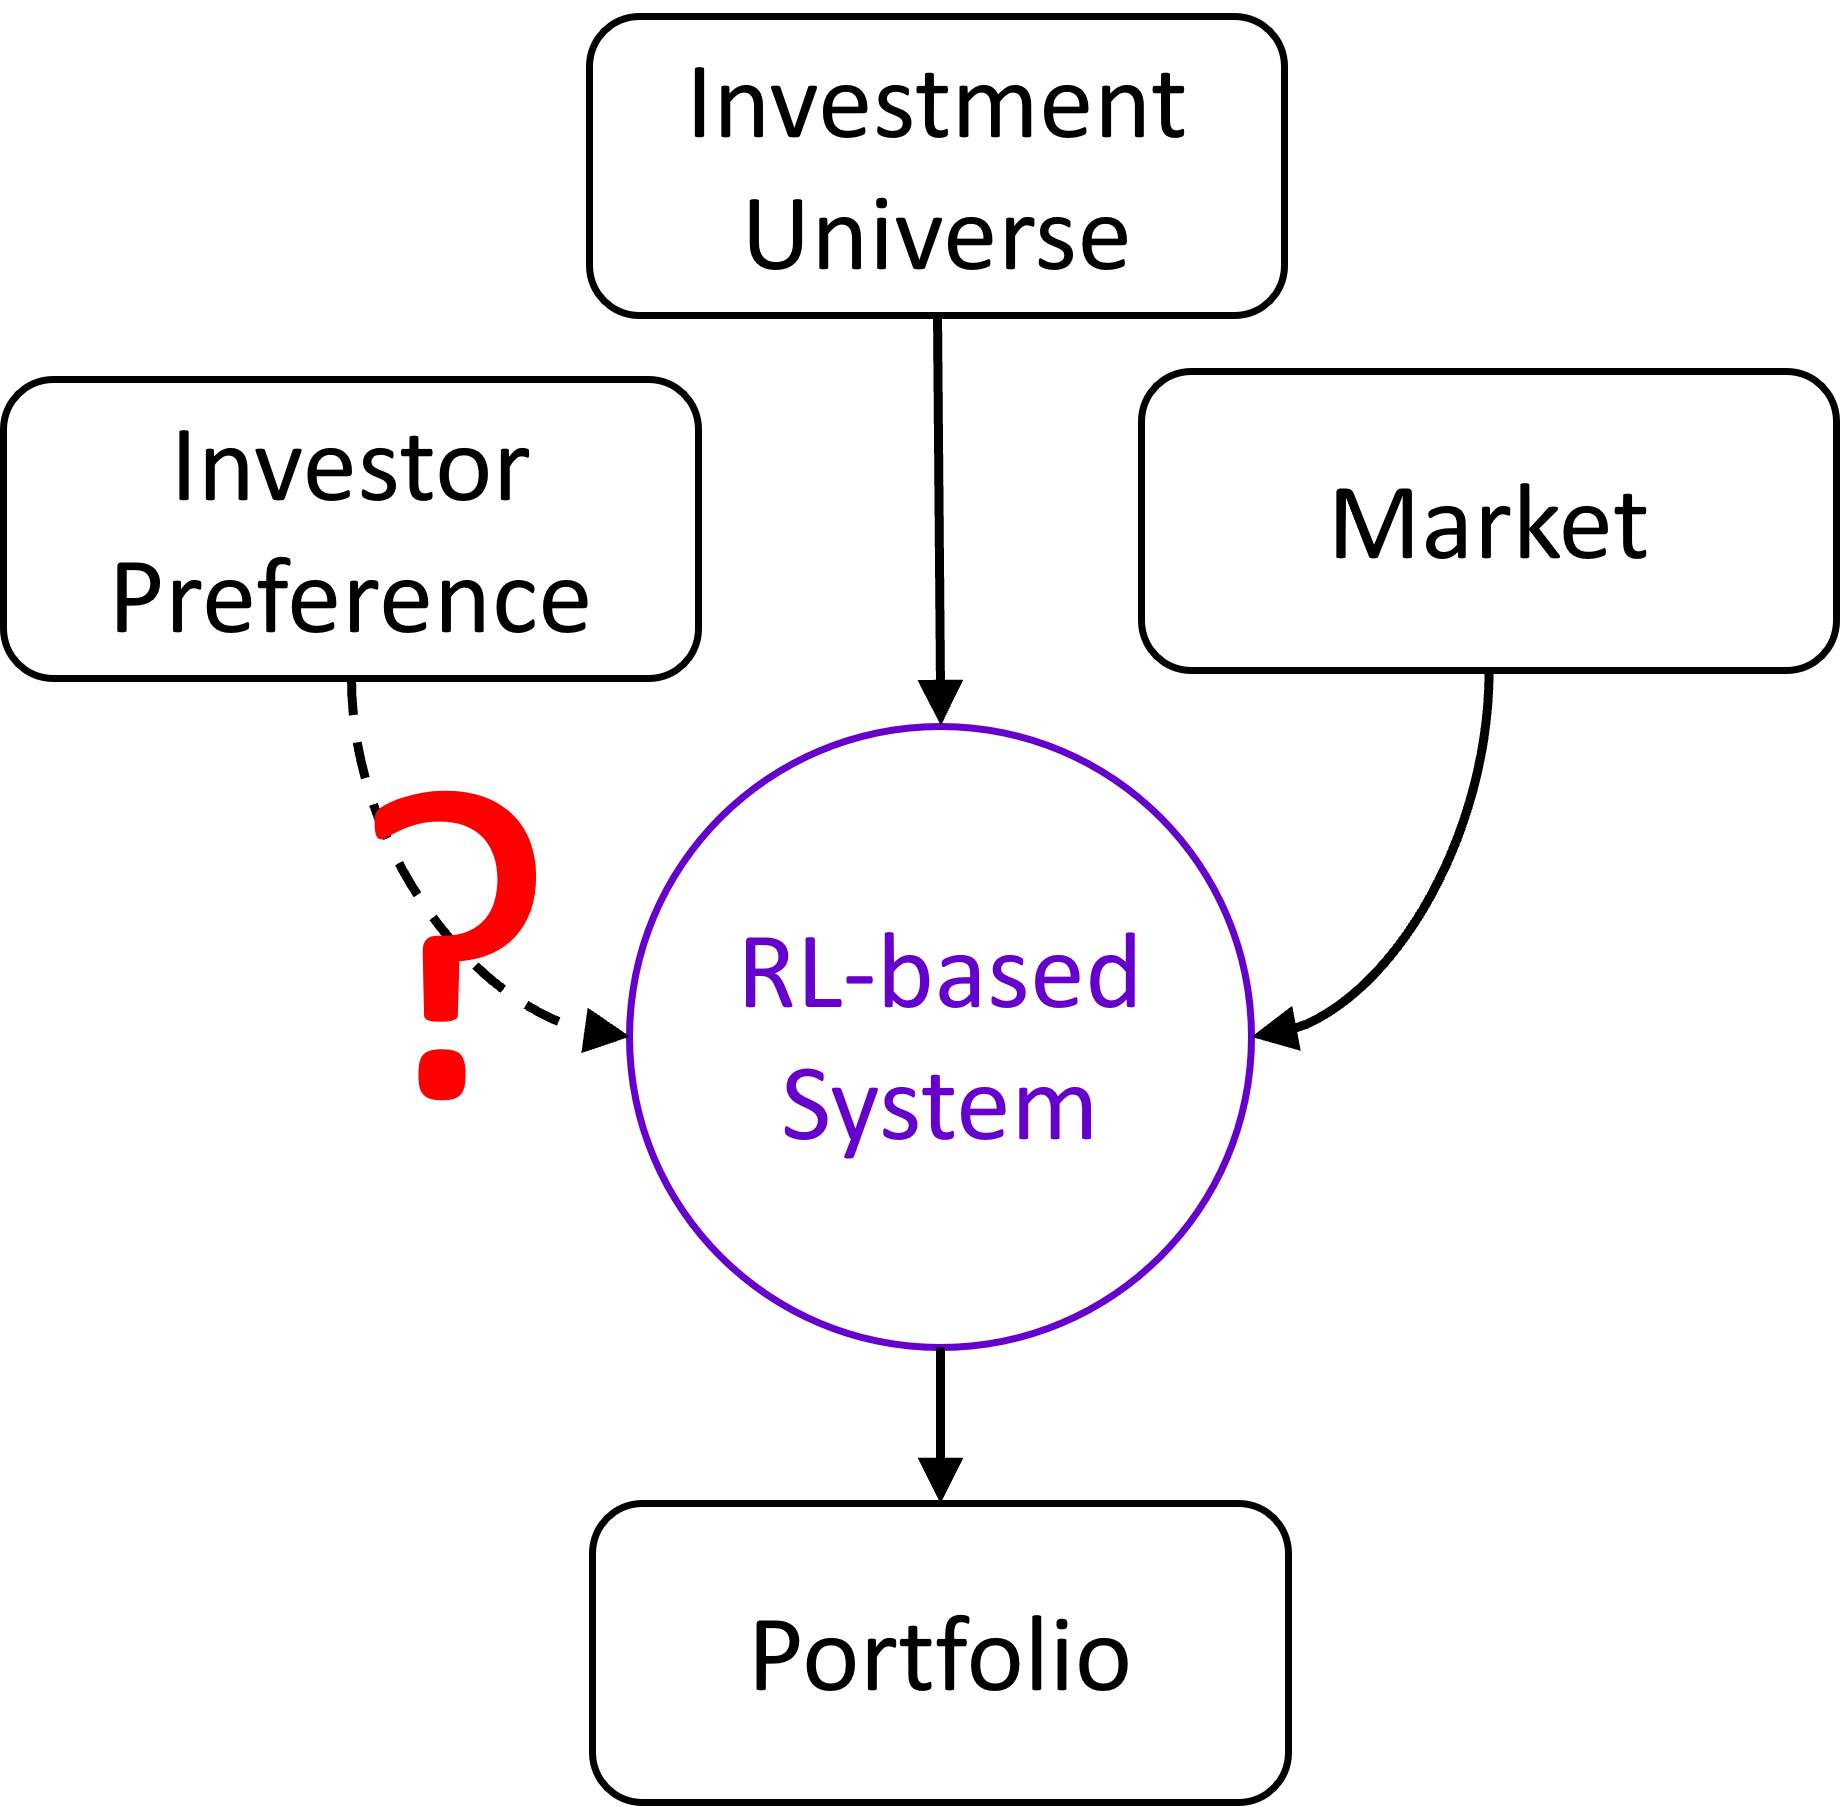
\includegraphics[width=4.8cm]{images/rl.png}
\end{center}
\end{column}
\end{columns}
\end{frame}






\begin{frame}
\frametitle{Objective}
\begin{columns}
\begin{column}{0.55\textwidth}
Our goal is to incorporate RL-based System with investor preference, \alert{investors' risk tolerance} in this case.

\end{column}
\begin{column}{0.45\textwidth}
\begin{center}
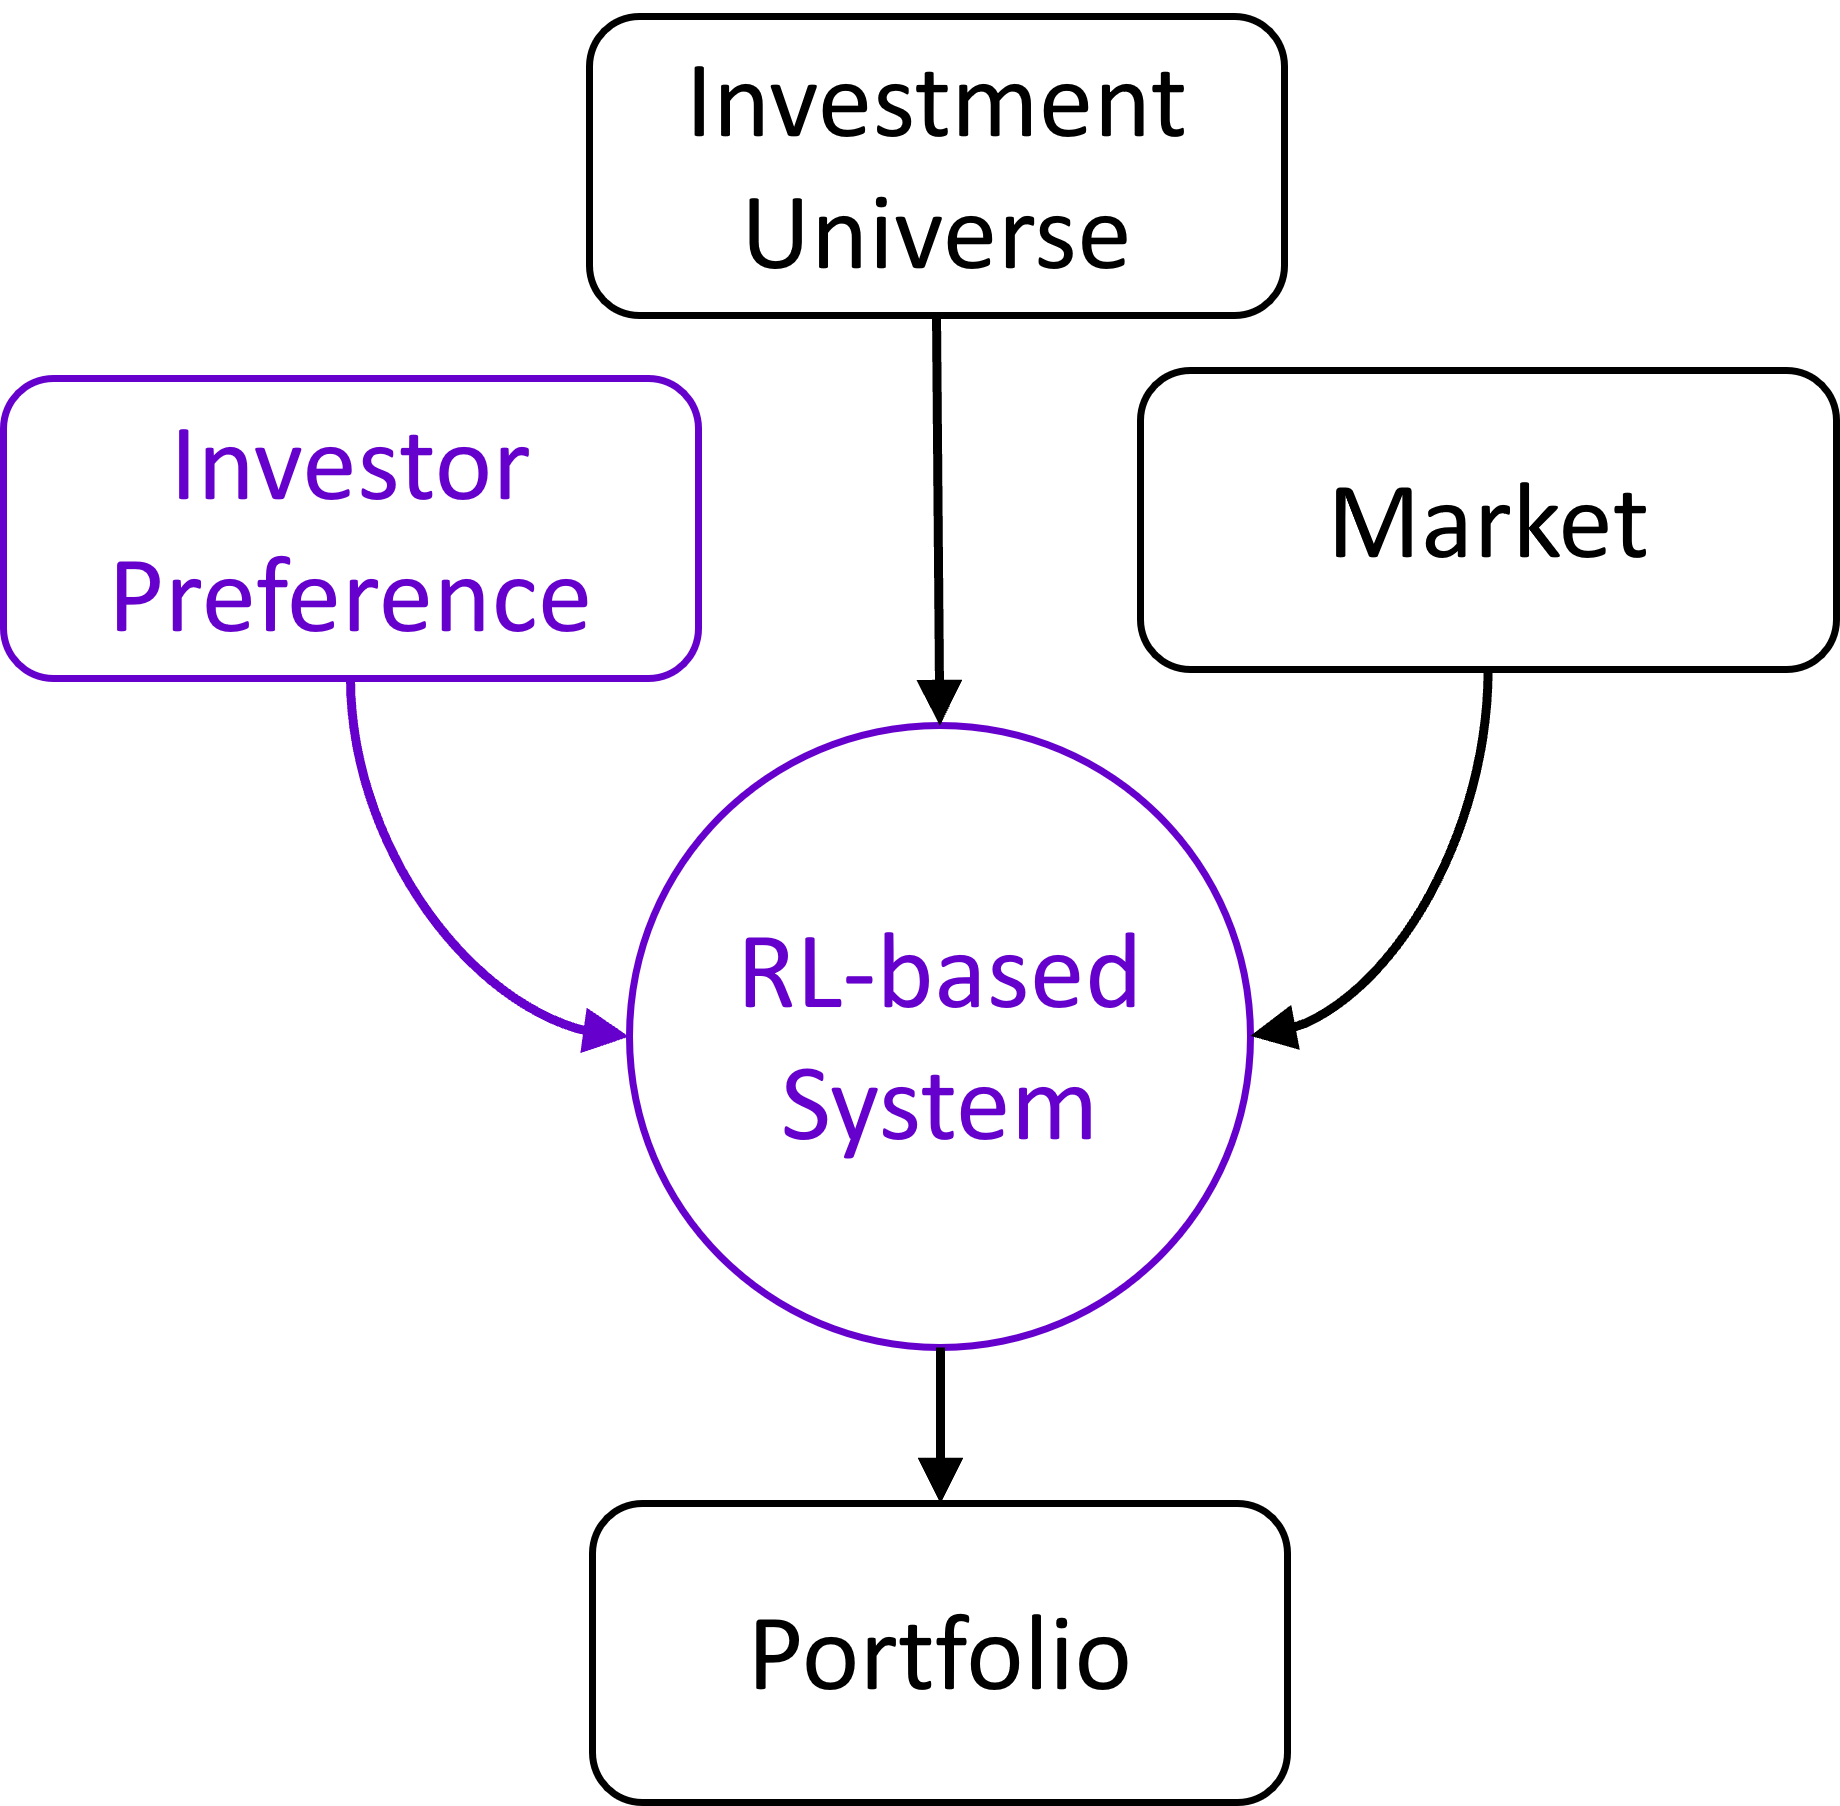
\includegraphics[width=4.8cm]{images/rl2.png}
\end{center}
\end{column}
\end{columns}
\end{frame}